\chapter{Background}
This chapter explains the methods and concepts these are separated in 3 parts one for basic knowledge, one for the evaluation methods used and one for the used models. 

\section{Basic Knowledge}
Important knowledge for the contents of the thesis mainly the what translation, automatic Speech recognition and dropout


\subsection{Automatic Speech Recognition}
Automatic speech recognition systems or short ASR systems are systems that recognise and transcribe spoken language. 

\todo{expand, explain, formulate}

\subsection{Translation}
Translation is the practice of translating text or language from one language into another language. This can be done by hand by a human or in a very statical approach where a dictionary is used to directly translate the text 

\todo{expand, explain, formulate}

\subsubsection{Speech translation}
Speech translation or spoken language translation is similar to the regular translation but it has, like the name says, spoken language as the basis instead of text. 
in Machine translation this is done either with cascaded models or en-to-end models 

\todo{expand, maybe citations, formulations}


\subsection{Dropout}
Monte-Carlo dropout is the process of masking neurons in a Deep Neural Network randomly, based on a Bayesian probability to 0. This is usually done during training to reduce the chance of the model overfitting on the trainings data \todo{add citation}
usually used in training 
- has been utilised in DNN to measure uncertainty
- mainly in Deep architectures but also in Auto-encoders
has been done as most NN outputs are deterministic so masking parts of the model with 0 should lead to different results with the same input as has been done in \cite{gal2016dropoutbayesianapproximationrepresenting}
-in ASR it has been tried here  \cite{8683086}
- in ASR it mainly stems from noisy audio 
\todo{fully formulate, add that one empty citation, potentially graphic?}

\subsection{Bayesian probabilities}
probability maths where conditional probabilities are used, esp. when working with conditional probability distributions.
\todo{explain the autoregressive manner used in these models, i.e., the probability of a generated token is based on the source sentence and the previous output prefixes.}

\subsection{Probabilites}
to get the probability of the model at the last layer after the input sequence  
take the softmax values at the last layer of the model to estimate quality (normal mode) for transctiption and transltation 
this all results in the formula $$p(y|x,\Theta)=\prod_{t=1}^T p(y_t|y_{<t}, x, \Theta) $$ where $\Theta$ is the model parameters, x is the input sequence, the softmax is used at every decoding step.
\todo{add example? }

\subsection{Entropy}
\label{entropy}
In Information theory the entropy is the amount of uncertainty or information that is in a probability distribution
The entropy is mathematically defined as $- \sum_{x\in \chi} p(x) log p(x)$ where p is a probability and $\chi$ is the probability distribution and x is an element from that probabilitiy distribution.
\todo{add citations, more explainations}
%TODO
\section{Evaluation metrics}
 for the evaluation of the results a couple of terms, algorithms, methods are used. 
 
\subsection{WER}
\label{wer}
The Word Error Rate, in short WER, has been proposed in \cite{woodard1982} and \cite{morris2004}.
It's based on the Levenshtein distance but instead of working on phonemes it operates on words.
The WER can be computed as $$WER=\frac{S+D+I}{N}=\frac{S+D+I}{S+D+C}$$ where S is the number of substitutions, D is the number of deletions, I is the number of insertions and N is the number of words in the reference and C is the number of correct words.

\subsection{Comet}
Comet, in full Crosslingual Optimized Metric for Evaluation of Translation, is a neuronal framework for machine translation evaluation that was proposed in \cite{rei-etal-2020-comet} 
for this thesis relevant is the Estimator model which used to estimate a quality score 
\todo{expand, explain more}

\subsection{Pearsoncorrelation}
method to see how correlated 2 sets of values are
is 1 if it's correlated and -1 if it's inversely correlated 
if it's 0 the sets are not correlated at all
\todo{citations, expand, more explainantions how it works}
%TODO

\section{Models}
All the models used in this thesis use a encoder-decoder architecture and specifically transformers
\subsection{Decoder-Encoder}
-Encoder-Decoder Models are Models that contain a Encoder, which creates an embedding for the model
and a Decoder, which decodes an embedding from the model into a form that is for example a human readable text. 
-the encoder output is then used as input for the decoder that produces the output of the model 
-Encoder-Decoder Architecture is used for Sequence-to-Sequence models esp. more complex/advanced Sequence-to-Sequence models 
\todo{
expand, add citations, maybe different graphics, add basic example
}

\tikzstyle{block} = [rectangle, draw, text width=3cm, text centered, minimum height=1.2cm, fill=blue!20]
\tikzstyle{arrow} = [thick,->,>=stealth]
\begin{figure}
    \centering
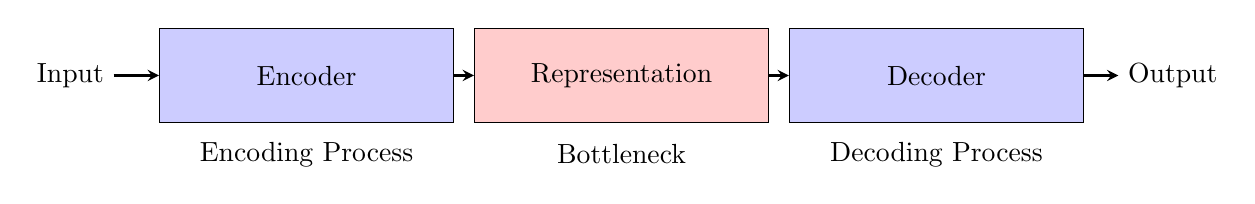
\begin{tikzpicture}
    % Nodes
    \node(input) [align=center] {Input};
    \node(encoder) [block, right of=input, xshift=2cm] {Encoder};
    \node(bottleneck) [block, right of=encoder, xshift=3cm, fill=red!20] {Representation};
    \node(decoder) [block, right of=bottleneck, xshift=3cm] {Decoder };
    \node (output) [align=center, right of=decoder, xshift=2cm] {Output};

    % Arrows
    \draw [arrow](input) -- (encoder);
    \draw [arrow] (encoder) -- (bottleneck);
    \draw [arrow] (bottleneck) -- (decoder);
    \draw [arrow] (decoder) -- (output);

    % Labels
    \node[below of=encoder] {Encoding Process};
    \node[below of=bottleneck] {Bottleneck};
    \node[below of=decoder] {Decoding Process};

\end{tikzpicture}
\label{fig:encoder-decoder model}
\caption{basic overview of a encoder-decoder model architecture}
\end{figure}

\subsection{Transformer}
Neural Network architecture that was first introduced in the paper Attention is all you need \cite{vaswani2023attentionneed} that makes use of self-attention mechanisms. 
It has a Encoder-Decoder structure whith N encoder blocks that are made up out of Multi-Head Attention blocks and feed forward networks both of which have a add and normalization layer behind that. 
The Decoder part consists of N blocks that contain a Masked multi-head attention block, a Multi-layer attention block and a feed forward neural network 
in the end there is a linear layer and a softmax layer

\begin{figure}
        \centering
        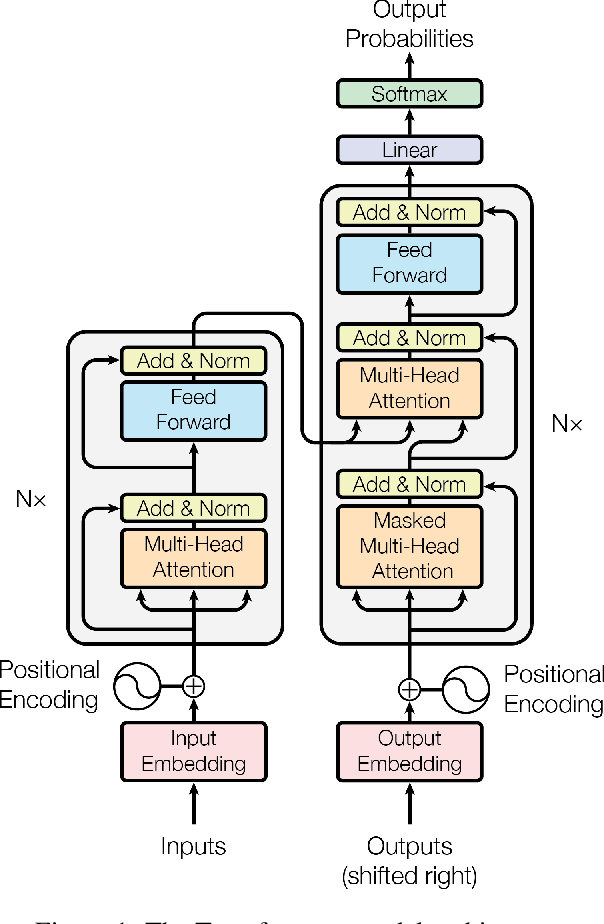
\includegraphics[width=0.5\linewidth]{Latex//sections//images/transformermodel.png}
        \caption{Transformer model architecture Vaswani et. all 2017}
        \label{fig:enter-label}
    \end{figure}

%TODO
\todo{add more, esp. more explainations}
\subsection{Cascaded Models}
Cascaded Speech translation Models consist of 2 parts a part that is responsible for transcribing the audio, which is usually done with an ASR model, and a part that is responsible for translating the resulting transcription, which is done with neural machine translation or statistical machine translation. 
%TODO citation and expand
\tikzstyle{block} = [rectangle, draw, text width=3.5cm, text centered, minimum height=1.2cm, fill=blue!20]
\tikzstyle{arrow} = [thick,->,>=stealth]
\tikzstyle{inputoutput} = [ellipse, draw, text width = 3.5cm, minimum height=1cm, text centered, fill=green!20]

\begin{figure}
    \centering
    

\begin{tikzpicture}
    
    % Nodes
    \node (input) [inputoutput] {Speech Input \\(Source Language)};
    \node (asr) [block, below of=input, node distance=3cm] {Automatic Speech \\ Recognition (ASR)};
    \node (translation) [block, right of=asr, node distance=5cm] {Text Translation \\ (e.g., MT model)};
    \node (output) [inputoutput, below of=translation, node distance=3cm] {Speech Output \\ (Target Language)};

    % Arrows (angled)
    \draw [arrow] (input) -- (asr);
    \draw [arrow] (asr) -- (translation);
    \draw [arrow] (translation) -- (output);

    % Labels for processes
    \node[below of=asr] {Speech Recognition};
    \node[below of=translation] {Text Translation};
    

\end{tikzpicture}
\label{fig:cascaded model}
\caption{Basic overview of a cascaded speech translation model}
\end{figure}
\subsection{End-to-End Models}
End-to-End Speech translation models do not have the explicit split between the Automatic Speech Recognition model and the translation, this means that such a model gets audio as an input and outputs the text in the target language. 
End-to-End models are trained to perform a task from the raw input, which in this case is audio, to the output, in this case the corresponding translation, without any intermediate processing from outside the model or feature-engineering in sub-models. 
%TODO citations, different architectures and expand
\subsection{Whisper}
Whisper is a multilingual multitask Model that is focused on speech processing and was proposes in the Robust Speech Recogintion via Large-Scale Weak Supervsion paper \cite{radford2022robust}. 
It's architecture is based on a classical Transformer Encoder-Decoder Architecture where the Transformer Encoder Blocks consist of self attention blocks and Multilayer perception blocks. 
The Transformer Decoder blocks use the learned position embeddings and tied input-output token representations. 
The encoder and decoder have the same number of transformer blocks .
The audio pre-processing is done by making sure the audio chunks that are then given to the model are 30 seconds long have ben sampled to 16,000 Hz and have a 80-channel log-magnitude Mel spectrogram representation, this log-mel spectrogramm is then computed with 25-milliseconf windows and a stride of 10 milliseconds. 
This input is then scaled to be between -1 and 1 and is but through 2 convolutional layers that have a filter width of 3 and use the GELU function as activation function, the second of those 2 layers has a stride of 2. 
The resulting data is then embedded with a sinusodial position embedding, which means %TODO
and put in the Encoder blocks. 

\begin{figure}
        \centering
        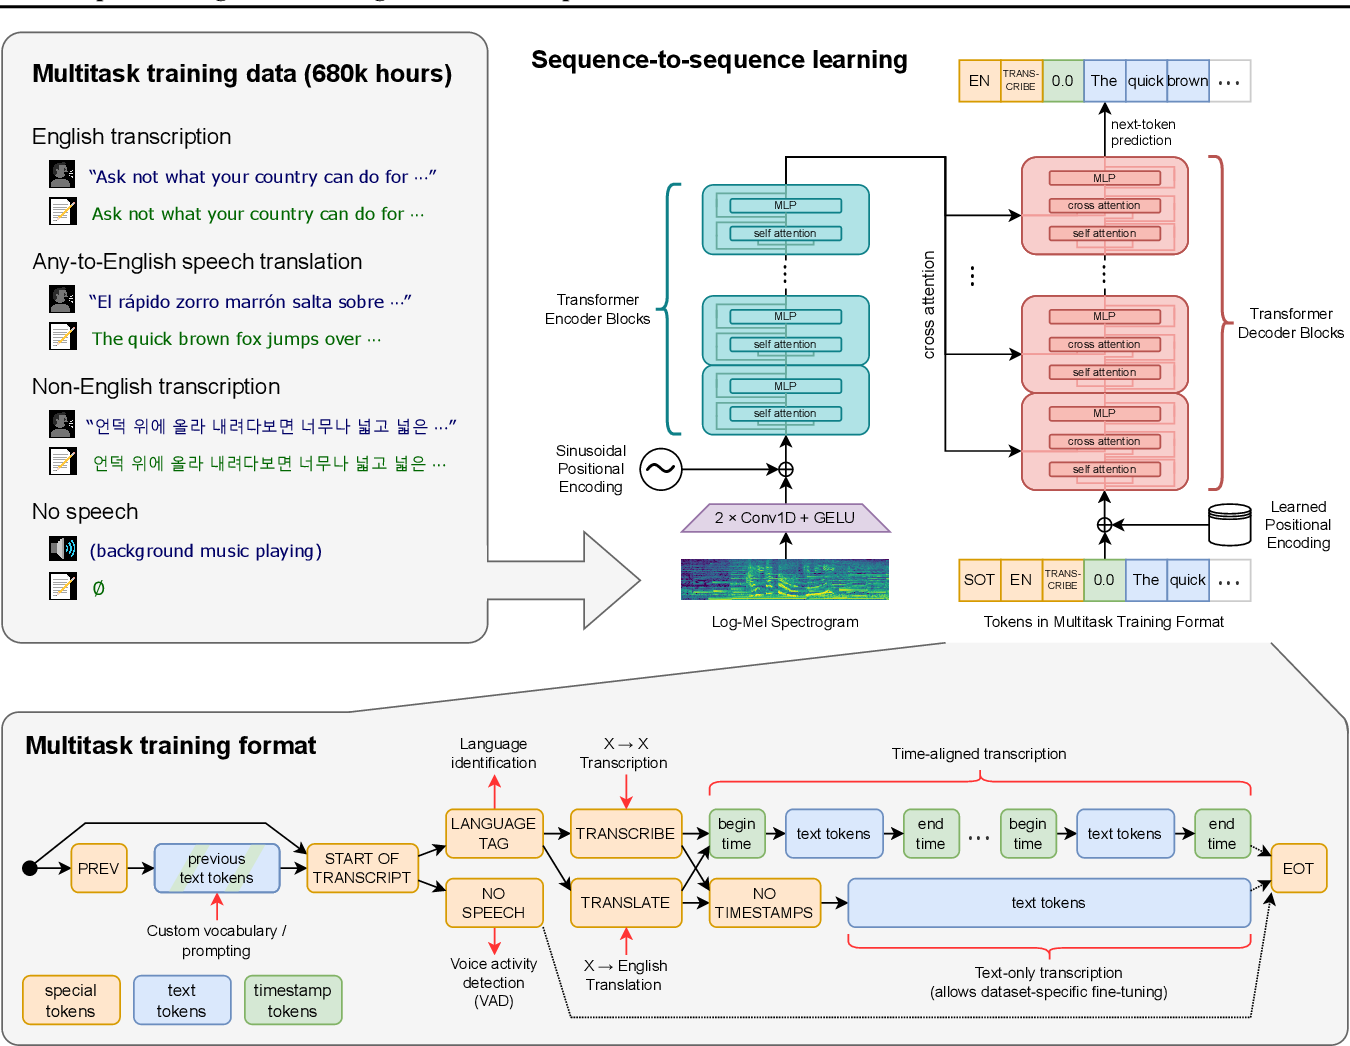
\includegraphics[width=0.5\linewidth]{Latex//sections//images/whispermodel.png}
        \caption{Overview of the Whisper architecture Radford et. al 2022}
        \label{fig:whispermodel}
    \end{figure}

%TODO
\subsection{Seamless}

Seamless is a Multimodal model 
experiments were run on \cite{seamless2023}, specifically the v2 large version which is an improved version of the SeamlessM4T model, 
of it both for the cascaded part and the end-to-end part

Seamless is a multilanagual multimodal model that uses a Transformer architecture. 
the architecture was proposed in \cite{seamless2023}
as the Transformer it is using a Encoder-Decoder architecture that in the v2 version uses a w2v-Bert speech encoder which was pretrained on unlabeled audio data. 
the general architecture is shown in \ref{fig:seamlessmodel}, for this thesis only the left half up to the Transformer Text decoder of the figure is relevant. 

\begin{figure}
        \centering
        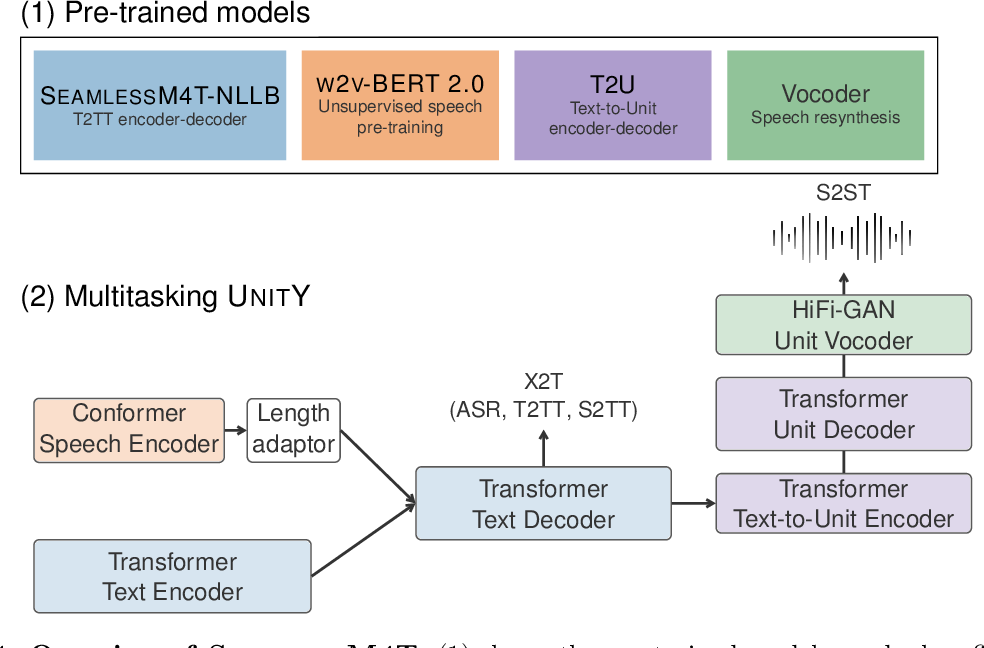
\includegraphics[width=0.5\linewidth]{Latex//sections/images/seamlessmodel.png}
        \caption{Overview of SeamlessM4T. (1) shows the pre-trained models used when finetuning multitasking UnitY. (2) outlines multitasking UnitY with its two encoders, text decoder, T2U encoder-decoder, and the supporting vocoders for synthesizing output speech in S2ST. \cite{seamless2023}(figure 4)}
        \label{fig:seamlessmodel}
\end{figure}
    
v2 uses a non autoregressive text to unit decoding which is the main difference to the first version however this change does not change much for this thesis as it only operates on Text-to-Text and Speech-to-text translation. 
The other change for v2 is that it uses a w2v-Bert 2.0 \cite{chung2021w2vbertcombiningcontrastivelearning} encoder that is trained self-supervised on 4.5 million hours of unlabled audio, as compared to the previous 1 million hours of unlabeled data. 
SeamlessM4T has been trained on unlabeled, human-labeled, pseudo-labled and automatically aligned data, where the text-to-text-translation (T2TT) was done on NLLB data \cite{nllbteam2022languageleftbehindscaling}
which is a method of creating low-resource language datasets with a combination of using flores \cite{guzmán2019floresevaluationdatasetslowresource} and NLLB Seed dataset, which is a set of professionally translated sentences in the wikipedia domain. 
% from seamless v2 paper
The X2T model, which can do T2TT, ASE and Speech to Text translation(S2TT), is trained on different sources of S2TT data that is human-labeled, pseudo-labeled and automatically aligned and is a combines the v2w-Bert model and the Text encoder from the NLLB T2TT model and the corresponding decoder.
It was trained in 2 steps on this data, the first one forcuses on supervised English ASR and S2TT data where the target langauge is English. 
The 2. step then focuses on english to X S2TT and non-English ASR data.


%TODO read further
\subsection{SentencePiece}
SentencePiece \cite{kudo-richardson-2018-sentencepiece} is a tokenizer and detokenizer that allows for subword units, especially byte pair-encoding \cite{sennrich-etal-2016-neural}, that are language independent as the sentences are treated as unicode character sequences and preprocessing is not always needed. 
It's comprised of a Normalizer, a Trainer, an Encoder and a Decoder. 
The Encoder uses the Normalizer to normalize the Test and then tokenizes the sentence. 
In the SentencePiece implementation the Decoding is considered the inverse operation of Encoding of normalized text, this results in a lossless tokenization, so there is no information loss over the process of encoding and decoding. 
To achieve this SentencePiece encodes white spaces with a meta-symbol that can be reverted. 
SentencePiece also manages the Vocabulary that is used in preprocessing as it also outputs a dictionary and can output a id sequence to text and vice versa mapping. 
As the SentencePiece model is self-contained it also leads to better reproducibility as only the model file is needed, which is publicly available. 

\subsection{DeltaLM}
DeltaLM is one of the current state of the art Neural Machine Translation models and the architectures that was proposed in \cite{ma2021deltalm}. 
It is based off of the classical Encoder-Decoder structure but both the encoder and decoder are initialised with the pretrained multilingual encoder. 
The training happens in a self-supervised manner. 

DeltaLM is considered one of the best text to text translation models. 

In addition to this is the Decoder a Interleaved Transformer Decoder, which is not the same architecture as the encoder and differs from the standard Transformer decoder in that the Transformerblocks now consist of a self-attention layer, two feed-forward networks and a cross-attention layer which are arranged as seen in \ref{fig:interleaved decoder}. 
This way of building the decoder is more similar to the structure of the encoder and makes it easier to leverage the pretrained encoder. 
The interleaved decoder is then initialised with the layers from the pretrained encoder, which is the InfoXLM \cite{chi2021infoxlminformationtheoreticframeworkcrosslingual}, in the following way, the self-attention and the bottom FFN layers are initialised wiht the odd layers of the InfoXLM encoder and the cross-attention and top FFN layers are initialised with the even layers. 
The leftover components of the decoder are also initialised the same as the pretrained encoder. 
This means that all of the sublayers are initialised with the pretrained weights and none of them use randomised names. 

%TODO
\begin{figure}
    \centering
    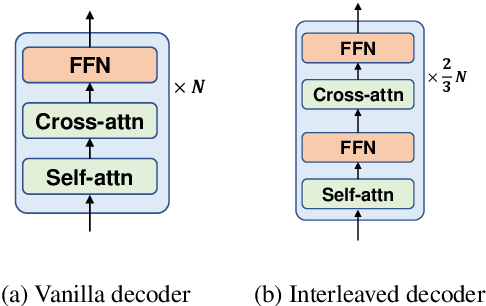
\includegraphics[width=0.5\linewidth]{Latex/sections/images/interleaveddecoder.png}
    \caption{Vanilla Transformer Decoder (left) compared to the interleaved Transformer decoder(right) from Ma et. al 2021}
    \label{fig:interleaved decoder}
    %source dlm paper
\end{figure}